\chapter{Análise e Desenho da Solução}
\label{cap:analise_desenho}

Neste capítulo descreve-se o processo de análise e o desenho da solução desenvolvida. Começa-se pelos requisitos, organizados segundo a abordagem \gls{FURPS+}, onde a dimensão \textit{Functionality} agrupa os requisitos funcionais e as restantes dimensões cobrem as propriedades de qualidade não funcionais. Em seguida, apresenta-se a análise do domínio que a solução tem de suportar, incluindo o modelo de aplicação e o modelo de domínio. A arquitetura é depois descrita com recurso à abordagem C4+1, combinando os níveis principais do modelo C4 \cite{C4Model} com uma vista física da infraestrutura. Por fim, apresentam-se o modelo de dados administrativo e o modelo de permissões que sustentam a autorização multiaplicação.

%----------------------------------------------------------------------------------------

\section{Requisitos}
\label{sec:requisitos}

Os requisitos da solução foram levantados a partir da especificação interna da empresa \cite{BackofficeSpec} e das discussões realizadas durante a fase de integração com a equipa. Para os organizar, adotou-se a abordagem \gls{FURPS+}, que classifica os requisitos de software em cinco dimensões principais, acrescentando ainda restrições adicionais de desenho, implementação ou operação \cite{Rashid2024FURPSMoSCoW}:

\begin{itemize}
  \item \textit{Functionality}: capacidades funcionais que o sistema deve disponibilizar.
  \item \textit{Usability}: aspetos da interface que afetam a utilização por operadores internos.
  \item \textit{Reliability}: capacidade de manter integridade, disponibilidade e comportamento previsível perante falhas ou operações inválidas.
  \item \textit{Performance}: tempos de resposta, carregamento inicial e impacto das operações sobre os recursos do sistema.
  \item \textit{Supportability}: manutenibilidade, testabilidade, modularidade e capacidade de adaptação da solução.
\end{itemize}

\noindent\textbf{Functionality}

Em vez de detalhar cada fluxo operacional isoladamente, os requisitos funcionais privilegiam aquilo que o sistema precisa de garantir para ser seguro, utilizável e evolutivo no contexto do ecossistema OnlyHighIQ. A organização seguinte relaciona-os com os objetivos definidos na introdução, usando o objetivo principal (OP) e os objetivos específicos OE1.1 a OE1.5 e OE2.1 a OE2.5.

\medskip\noindent\textit{Autenticação, autorização e administração}: este grupo concretiza sobretudo os objetivos OE1.1, OE1.2 e OE1.3, porque define a base comum de identidade, autorização e gestão de operadores reutilizável por várias aplicações.

\begin{itemize}
  \item \textbf{RF01}: o painel deve autenticar operadores internos através do AWS Cognito, com gestão de sessão e suporte a \gls{MFA}.
  \item \textbf{RF02}: após a autenticação, o sistema deve resolver o contexto interno do operador, incluindo perfis atribuídos, aplicações acessíveis e permissões efetivas.
  \item \textbf{RF03}: o acesso ao backoffice de gestão e ao painel operacional da JustCauses deve ser separado por aplicação, impedindo a entrada em áreas não autorizadas.
  \item \textbf{RF04}: o sistema deve controlar o acesso a páginas com base em guardas de rota e em regras configuráveis por página.
  \item \textbf{RF05}: as permissões exigidas por cada página devem poder ser alteradas sem nova publicação da aplicação.
  \item \textbf{RF06}: todos os endpoints sensíveis da \gls{API} devem validar permissões no servidor antes de executar qualquer operação.
  \item \textbf{RF07}: o painel deve disponibilizar mecanismos de gestão administrativa para contas internas, perfis de acesso, permissões por aplicação e configuração do modelo de autorização.
\end{itemize}

\medskip\noindent\textit{Operação da plataforma}: este grupo concretiza sobretudo os objetivos OE2.1 a OE2.5, aplicando a estrutura comum à primeira aplicação integrada no ecossistema.

\begin{itemize}
  \item \textbf{RF08}: o painel deve disponibilizar um \textit{dashboard} com métricas operacionais relevantes e indicadores de atividade da plataforma.
  \item \textbf{RF09}: o painel deve suportar a revisão do ciclo de vida das campanhas, incluindo estados de aprovação, rejeição e pedido de alterações.
  \item \textbf{RF10}: o painel deve permitir criar, editar e desativar categorias de campanhas.
  \item \textbf{RF11}: o painel deve suportar a verificação \gls{KYC} de utilizadores individuais e a verificação \gls{KYB} de organizações, incluindo consulta de dados submetidos, decisão administrativa, notificação e auditoria.
  \item \textbf{RF12}: a arquitetura deve permitir incorporar outros fluxos operacionais do ecossistema sem alterar o núcleo do mecanismo de autorização.
\end{itemize}

\medskip\noindent\textit{Rastreabilidade}: este grupo apoia simultaneamente o OP e o OE1.4, uma vez que a auditoria é uma capacidade transversal necessária para administrar aplicações internas com responsabilização.

\begin{itemize}
  \item \textbf{RF13}: o painel deve manter um registo imutável das ações relevantes e das tentativas de acesso negado, consultável por filtros de data, operador e tipo de evento.
\end{itemize}

A Tabela~\ref{tab:mapeamento_objetivos_requisitos} resume a relação entre objetivos e requisitos.

\begin{table}[H]
\caption{Relação entre objetivos e requisitos}
\label{tab:mapeamento_objetivos_requisitos}
\begin{center}
\small
\begin{tabular}{|p{2.2cm}|p{5.2cm}|p{5.4cm}|}
\hline
\textbf{Objetivo} & \textbf{Foco} & \textbf{Requisitos associados} \\ \hline
OP & Base comum de backoffice multiaplicação & RF01 a RF13 e RNF01 a RNF16 \\ \hline
OE1.1 & Autenticação e contexto administrativo do operador & RF01, RF02, RNF04 \\ \hline
OE1.2 & Perfis e permissões por aplicação & RF03, RF07, RNF05, RNF14 \\ \hline
OE1.3 & Controlo de acesso em aplicação, página, interface e \gls{API} & RF04, RF05, RF06, RNF12 \\ \hline
OE1.4 & Auditoria, acessos negados e atividade dos operadores & RF13, RNF06, RNF10 \\ \hline
OE1.5 & Arquitetura e persistência extensíveis & RF12, RNF11, RNF13, RNF14, RNF15, RNF16 \\ \hline
OE2.1 & Integração da JustCauses como primeira aplicação operacional & RF03, RF08, RF12 \\ \hline
OE2.2 & Revisão de campanhas e notificação associada & RF09, RF13 \\ \hline
OE2.3 & Gestão de categorias e dados operacionais & RF10 \\ \hline
OE2.4 & Dashboard, analytics e indicadores operacionais & RF08 \\ \hline
OE2.5 & Verificação de identidade e oficialidade & RF11, RF13 \\ \hline
\end{tabular}
\end{center}
\end{table}

\noindent\textbf{Usability}
\begin{itemize}
  \item \textbf{RNF01}: a interface deve ser utilizável por operadores sem formação técnica, com navegação clara entre módulos e separação visível entre aplicações.
  \item \textbf{RNF02}: ações indisponíveis para o operador devem ser omitidas ou bloqueadas de forma explícita, para que a interface não sugira operações não autorizadas.
  \item \textbf{RNF03}: operações críticas devem apresentar mensagens claras de confirmação, erro ou acesso negado.
\end{itemize}

\noindent\textbf{Reliability}
\begin{itemize}
  \item \textbf{RNF04}: toda a comunicação deve ser feita sobre HTTPS, com autenticação obrigatória nos pontos de entrada do painel e suporte a \gls{MFA} via AWS Cognito.
  \item \textbf{RNF05}: as validações de servidor devem rejeitar operações que violem o modelo de autorização, incluindo permissões associadas à aplicação errada ou múltiplos perfis da mesma aplicação.
  \item \textbf{RNF06}: os registos de auditoria devem ser imutáveis e associados a exatamente um operador interno, evitando registos anónimos no contexto administrativo.
  \item \textbf{RNF07}: o sistema deve utilizar os mecanismos de disponibilidade e monitorização da infraestrutura AWS, nomeadamente CloudWatch para observabilidade.
\end{itemize}

\noindent\textbf{Performance}
\begin{itemize}
  \item \textbf{RNF08}: as respostas da \gls{API} para operações de leitura devem ter uma latência inferior a 500 ms em condições normais.
  \item \textbf{RNF09}: o carregamento inicial do painel deve ocorrer em menos de 3 segundos em condições normais de utilização.
  \item \textbf{RNF10}: o módulo de auditoria deve absorver picos de escrita sem degradar o desempenho da base relacional usada pelos dados operacionais da JustCauses.
\end{itemize}

\noindent\textbf{Supportability}
\begin{itemize}
  \item \textbf{RNF11}: o código deve manter separação clara entre interface, rotas, controladores, serviços, repositórios e configuração de infraestrutura.
  \item \textbf{RNF12}: a configuração de \textit{page gates}, isto é, regras de acesso por página, deve poder ser alterada sem nova publicação da aplicação, permitindo adaptar acessos por aplicação e por página.
  \item \textbf{RNF13}: a solução deve manter contratos de \gls{API} estáveis e identificadores de interface adequados à validação manual e aos testes de qualidade existentes.
\end{itemize}

\noindent\textbf{+ Escalabilidade e restrições}
\begin{itemize}
  \item \textbf{RNF14}: o modelo de autorização deve permitir acrescentar futuras aplicações sem redesenhar o núcleo do backoffice, recorrendo a perfis e permissões associados a cada aplicação.
  \item \textbf{RNF15}: operadores, perfis, permissões, \textit{page gates} e auditoria devem permanecer separados dos dados transacionais da JustCauses.
  \item \textbf{RNF16}: a solução deve respeitar a base tecnológica definida pela empresa, incluindo React, Node.js/Express, AWS Cognito, S3, SES, CloudWatch, PostgreSQL, DynamoDB e o processo de entrega com \gls{CI/CD}.
\end{itemize}

%----------------------------------------------------------------------------------------

\section{Análise}
\label{sec:analise_dominio}

O painel de administração opera sobre dois níveis de domínio. O primeiro corresponde aos conceitos transversais do próprio backoffice, como operador interno, aplicação, perfil de acesso, permissão e registo de auditoria. O segundo corresponde ao domínio operacional da JustCauses, que é a primeira aplicação integrada no sistema. Esta distinção é importante porque o relatório não descreve apenas um painel isolado da JustCauses: descreve uma base de administração multiaplicação, onde a JustCauses é o primeiro caso operacional completo.

\subsection{Modelo de aplicação}
\label{subsec:modelo_aplicacao}

O modelo de aplicação traduz os conceitos de domínio que a arquitetura precisa de suportar. No estado atual existem duas áreas funcionais: o backoffice transversal, usado para administração interna, e a JustCauses, primeira aplicação operacional integrada. A Tabela~\ref{tab:entidades_dominio} apresenta as principais entidades e o seu papel.

\begin{table}[H]
\caption{Principais entidades do modelo de aplicação}
\label{tab:entidades_dominio}
\begin{center}
\footnotesize
\begin{tabular}{|l|p{9cm}|}
\hline
\textbf{Entidade} & \textbf{Descrição} \\ \hline
Aplicação         & Área funcional administrada pelo backoffice. No estado atual, existem o backoffice transversal e a aplicação JustCauses, estando o modelo preparado para futuras aplicações. \\ \hline
Operador interno  & Utilizador autorizado a aceder ao backoffice, autenticado via Cognito e associado internamente a perfis de acesso. \\ \hline
Perfil de acesso  & Conjunto de permissões associado a uma aplicação. Um operador pode ter, no máximo, um perfil por aplicação, exceto quando tem um perfil global de backoffice. \\ \hline
Permissão         & Capacidade granular que autoriza uma ação ou consulta. Cada permissão pertence a uma aplicação e só pode ser atribuída a perfis dessa aplicação. \\ \hline
\textit{Page gate} & Configuração que define que permissões permitem abrir uma página do backoffice ou de uma aplicação integrada. \\ \hline
Registo de auditoria & Entrada imutável que documenta uma ação de um operador sobre uma entidade crítica da plataforma, com marca temporal e identificação do responsável. \\ \hline
Utilizador individual & Conta pessoal registada na plataforma JustCauses, com perfil próprio, estado de conta e processo de verificação de identidade associado. \\ \hline
Organização       & Perfil coletivo que pode criar campanhas em nome de uma entidade, com dados de identificação, estado operacional e processo de verificação próprio (\gls{KYB}). \\ \hline
Criador           & Abstração usada para representar quem submete campanhas na JustCauses. Pode corresponder a um utilizador individual ou a uma organização, consoante a natureza do perfil. \\ \hline
Campanha          & Projeto de angariação de fundos submetido por um criador, com ciclo de vida acompanhado pelo painel. \\ \hline
Thread de revisão & Sequência de revisão associada a uma campanha ou alteração submetida, permitindo ao operador aprovar, rejeitar ou pedir correções sem perder o histórico da decisão. \\ \hline
Categoria         & Etiqueta temática associada a campanhas, gerida exclusivamente pelo painel de administração. \\ \hline
Doação            & Contribuição financeira de um utilizador para uma campanha, consultável para acompanhamento operacional. \\ \hline
Depósito          & Entrada financeira no sistema partilhado de pagamentos, usada para acompanhar fundos recebidos antes da sua distribuição operacional. \\ \hline
Transação         & Movimento financeiro registado no sistema, incluindo pagamentos, transferências e outros eventos relevantes para rastreabilidade financeira. \\ \hline
Levantamento      & Pedido de transferência dos fundos angariados por um criador, sujeito a validação e aprovação manual pelo operador. \\ \hline
Verificação KYC   & Processo de validação de identidade de um utilizador individual, comparando dados do perfil com dados de verificação recebidos do fornecedor externo. \\ \hline
Submissão KYB     & Conjunto de documentos e decisão administrativa usados para validar a oficialidade de uma organização e a representação associada. \\ \hline
Documento de verificação & Ficheiro submetido no âmbito de \gls{KYC} ou \gls{KYB}, armazenado externamente e consultado pelo operador quando necessário para a decisão. \\ \hline
Denúncia          & Reporte de conteúdo inadequado submetido por um utilizador para revisão pelo operador do painel. \\ \hline
\end{tabular}
\end{center}
\end{table}

Depois da Tabela~\ref{tab:entidades_dominio}, o aspeto essencial é a separação entre conceitos transversais e conceitos específicos da JustCauses. Aplicação, operador, perfil, permissão, \textit{page gate} e auditoria são reutilizáveis; utilizadores individuais, organizações, criadores, campanhas, threads de revisão, categorias, doações, depósitos, transações, levantamentos e verificações pertencem ao domínio operacional da JustCauses. O conceito de criador evita duplicar regras entre pessoas e organizações: ambos podem submeter campanhas, mas a validação que lhes é aplicável é diferente. Os utilizadores individuais são avaliados por \gls{KYC}; as organizações são avaliadas por \gls{KYB}. Esta distinção também ajuda a perceber porque é que a arquitetura não deve misturar a configuração do backoffice com os dados de negócio de cada aplicação integrada.

A Figura~\ref{fig:domain_model} apresenta esta separação no modelo de domínio usado como referência para o desenho da solução.

\IfFileExists{frontmatter/assets/backoffice/ch3/uml/architecture/domain-model.png}{
\begin{figure}[H]
\centering
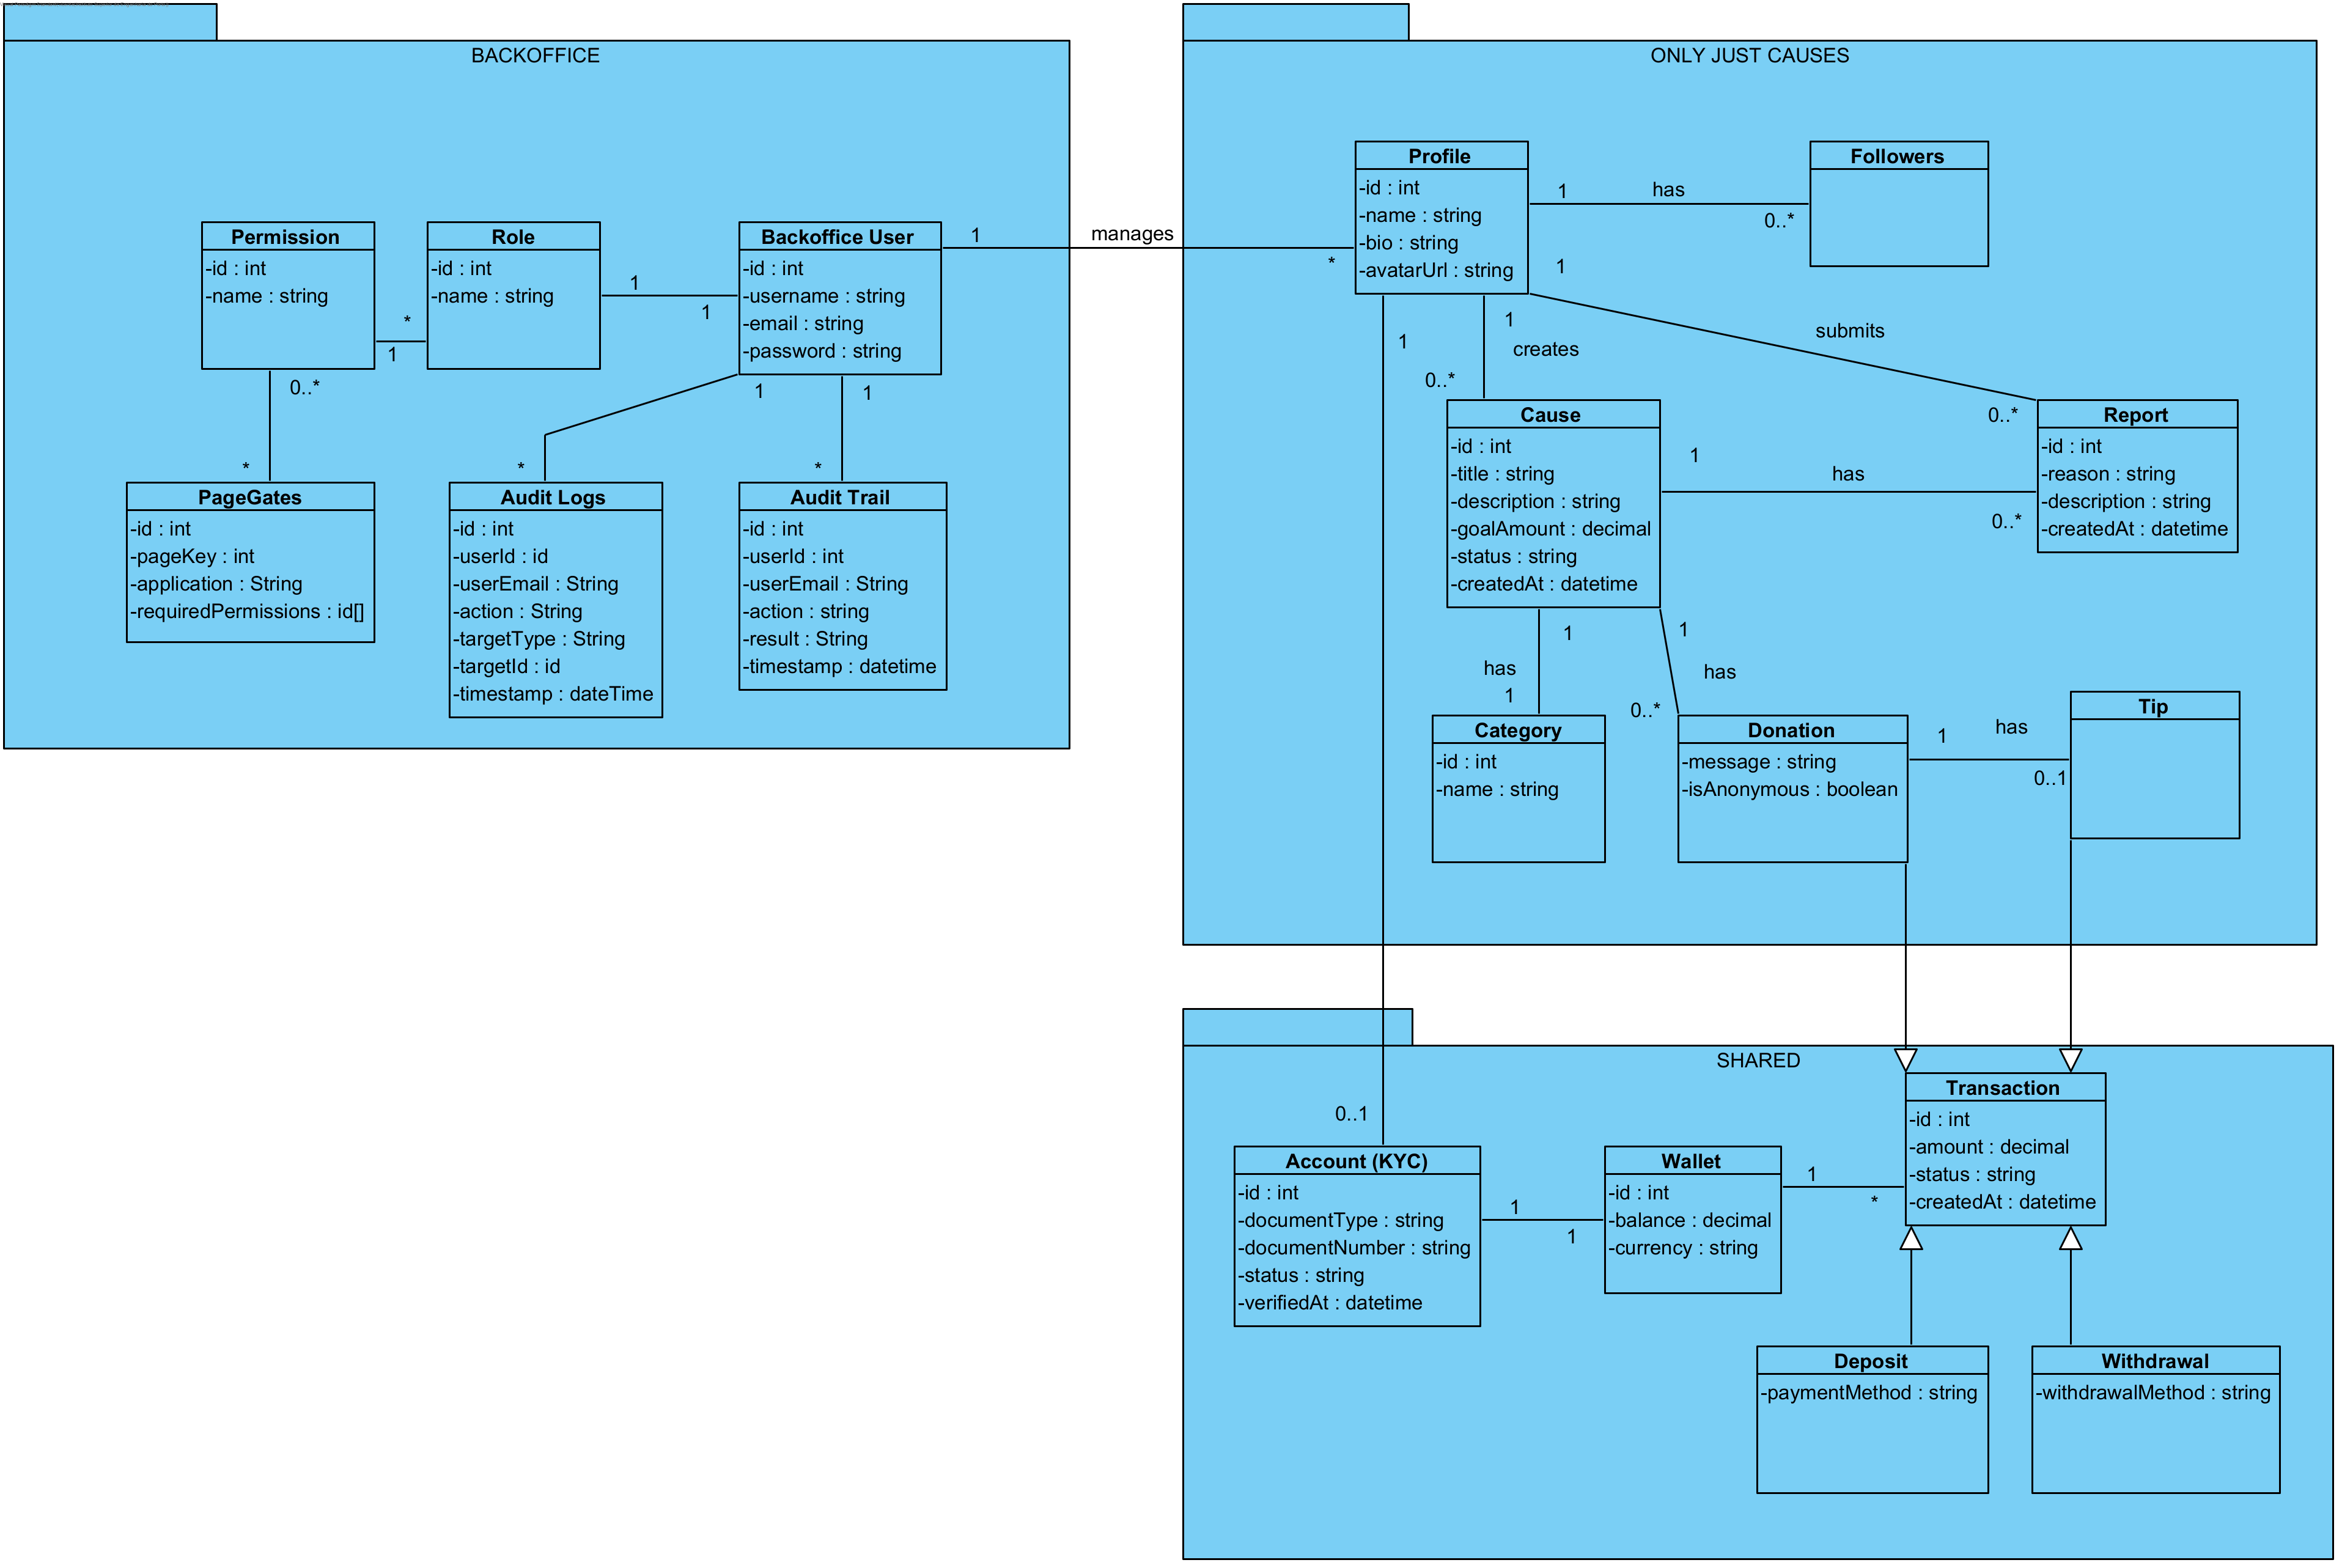
\includegraphics[width=0.95\textwidth, height=0.82\textheight, keepaspectratio]{frontmatter/assets/backoffice/ch3/uml/architecture/domain-model.png}
\caption{Modelo de domínio do backoffice e da JustCauses}
\label{fig:domain_model}
\end{figure}

Depois da Figura~\ref{fig:domain_model}, a leitura pretendida é que o backoffice administra entidades da JustCauses, mas mantém o seu próprio domínio de acesso e auditoria separado. No bloco de backoffice surgem as entidades que suportam autorização e auditoria. No bloco Only Just Causes surgem perfis, organizações, campanhas, categorias, verificações, doações, denúncias e relações de acompanhamento. No bloco partilhado surgem contas, carteiras e movimentos financeiros, incluindo depósitos e levantamentos.
}{}

%----------------------------------------------------------------------------------------

\section{Arquitetura da solução}
\label{sec:arquitetura}

A arquitetura do painel de administração foi definida com base nos requisitos levantados e nas restrições de infraestrutura já existentes no ecossistema da OnlyHighIQ. Para a descrever de forma estruturada, adotou-se uma abordagem C4+1: os níveis C4 principais \cite{C4Model}, que organizam a descrição em contexto do sistema, contentores e componentes, são complementados por uma vista física da infraestrutura. Esta extensão é útil porque o comportamento do backoffice depende também da forma como autenticação, distribuição, computação, persistência e observabilidade estão implantadas na AWS.

\subsection{Nível 1: contexto do sistema}

O painel de administração é um sistema de uso exclusivamente interno, acedido por operadores autorizados da OnlyHighIQ através de um navegador \textit{web}. No nível de contexto, a dependência externa mais relevante para a entrada no sistema é o AWS Cognito, responsável pela autenticação dos operadores. As restantes dependências, como bases de dados, serviços de armazenamento, e-mail transacional e observabilidade, são detalhadas nos níveis seguintes da arquitetura.

A Figura~\ref{fig:c4_level1} mostra o backoffice como sistema interno acedido pela interface de utilizador e integrado com o AWS Cognito para autenticação.

\begin{figure}[H]
\centering
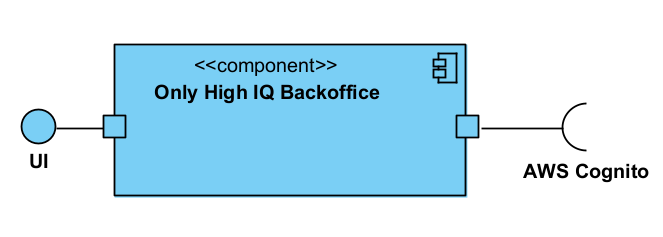
\includegraphics[width=0.95\textwidth, height=0.85\textheight, keepaspectratio]{frontmatter/assets/backoffice/docs/C4-Level1.png}
\caption{Diagrama de contexto: C4 Nível 1}
\label{fig:c4_level1}
\end{figure}

Depois da Figura~\ref{fig:c4_level1}, o ponto a reter é que o backoffice se posiciona como aplicação administrativa interna. O operador não comunica diretamente com os dados da JustCauses ou com serviços de suporte: entra primeiro no painel, autentica-se através do Cognito e só depois executa operações sujeitas ao modelo de autorização descrito nas secções seguintes.

\subsection{Nível 2: contentores e vista física}

O sistema é composto por dois contentores principais: a aplicação \textit{front-end}, desenvolvida em React 19 com TypeScript e Vite, e a \gls{API} \textit{back-end}, desenvolvida em Node.js com Express 5 e TypeScript. A comunicação entre os dois é feita exclusivamente via \gls{REST} sobre HTTPS, com autenticação baseada em tokens JWT emitidos pelo AWS Cognito e validados pelo \textit{back-end} em cada pedido.

A Figura~\ref{fig:c4_level2} evidencia a separação entre interface, \gls{API}, bases de dados e serviços externos. O ponto a reter deste nível é que o \textit{front-end} consome a \gls{API}; não acede diretamente às bases de dados nem decide sozinho autorizações sensíveis.

\begin{figure}[H]
\centering

\includegraphics[width=0.95\textwidth, height=0.85\textheight, keepaspectratio]{frontmatter/assets/backoffice/docs/C4-Level2.png}
\caption{Diagrama de contentores: C4 Nível 2}
\label{fig:c4_level2}
\end{figure}

Depois da Figura~\ref{fig:c4_level2}, a leitura pretendida é a separação de responsabilidades. O navegador apresenta a interface e envia pedidos autenticados; a \gls{API} concentra a validação de tokens, permissões e regras de negócio; o DynamoDB guarda a configuração e a auditoria próprias do backoffice; e as bases Aurora PostgreSQL mantêm os dados operacionais da JustCauses e os dados partilhados do ecossistema. Esta opção suporta uma arquitetura multiaplicação sem criar um backoffice isolado para cada produto.

A camada de persistência é composta por três áreas com responsabilidades distintas: a base Aurora PostgreSQL da JustCauses para dados operacionais da aplicação, a base Aurora PostgreSQL partilhada para entidades comuns do ecossistema, e o AWS DynamoDB para os dados de configuração e rastreabilidade do painel (perfis, permissões, configuração de acesso por rota e registos de auditoria). O acesso a ficheiros, como documentos de \gls{KYC}, documentos de \gls{KYB} e imagens de campanhas, é feito via AWS S3.

\subsubsection{Vista física}
\label{subsec:vista_fisica}

A infraestrutura do painel de administração reside integralmente na \gls{AWS} e usa o conjunto de serviços geridos já adotado pelo ecossistema da \textit{OnlyHighIQ}. A Figura~\ref{fig:vista_fisica} apresenta a vista física da solução, desde a filtragem de tráfego por \gls{WAF} e a distribuição via CloudFront, passando pela autenticação com Cognito, até à execução do \textit{back-end} em instâncias Spot com Auto Scaling distribuídas por três zonas de disponibilidade e à persistência em Aurora Multi-AZ e DynamoDB.

\begin{figure}[H]
\centering
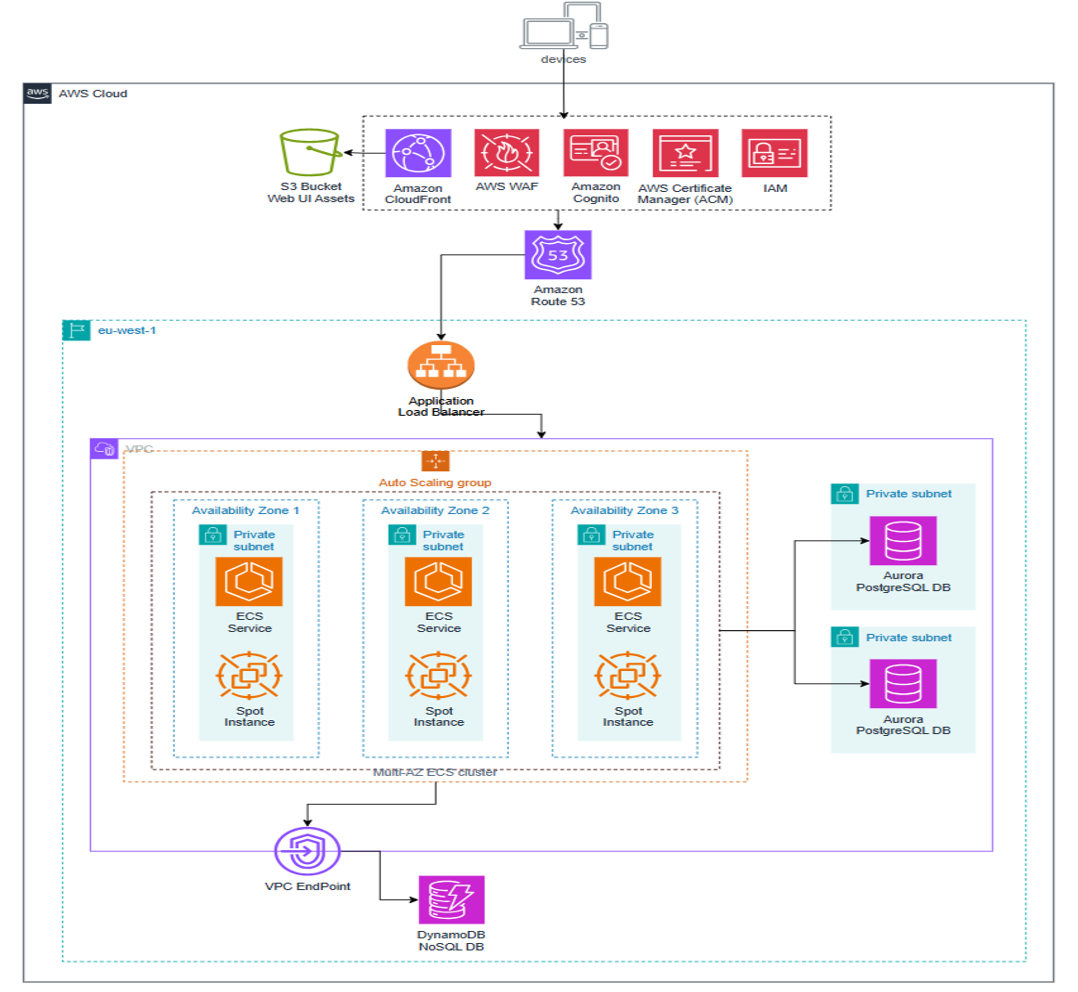
\includegraphics[width=0.95\textwidth, height=0.85\textheight, keepaspectratio]{frontmatter/assets/backoffice/docs/aws-physical-view.png}
\caption{Vista física da infraestrutura AWS do backoffice}
\label{fig:vista_fisica}
\end{figure}

A camada de borda (Route 53, CloudFront com S3, \gls{WAF} e ACM) segue o padrão já estabelecido no ecossistema da \textit{OnlyHighIQ} e não introduz lógica específica do backoffice. O serviço com impacto direto no painel é o Amazon Cognito: gere a identidade dos operadores com \gls{MFA}, emite tokens JWT e organiza utilizadores em grupos que mapeiam para os perfis do painel. O \textit{back-end} valida esses tokens com o \gls{JWKS} público do Cognito sem armazenar credenciais localmente, mantendo a fonte de verdade da identidade fora da aplicação.

Na computação, o servidor Node.js corre em contentores geridos pelo Amazon ECS com instâncias Spot, distribuídos por um grupo de Auto Scaling em três zonas de disponibilidade, combinando custo reduzido com resiliência a falhas de zona.

Na persistência, o Amazon Aurora PostgreSQL armazena os dados relacionais da JustCauses com replicação Multi-AZ. O Amazon DynamoDB é dedicado exclusivamente aos dados de controlo e rastreabilidade do backoffice: utilizadores internos, perfis, permissões, configuração de page gates e registos de auditoria (\texttt{BO\_Users}, \texttt{BO\_Roles}, \texttt{BO\_Permissions}, \texttt{BO\_PageGates}, \texttt{BO\_Logs}). Este acesso é feito através de um VPC Endpoint privado, sem tráfego pela internet pública. A separação entre os dados operacionais da JustCauses e os dados administrativos do painel é uma decisão deliberada: garante que auditoria e configuração de acesso não concorrem com as entidades da plataforma. O Amazon SES completa esta camada ao enviar notificações automáticas a criadores em resposta a decisões do painel, como revisões de campanhas ou alterações de estado de conta.

A Tabela~\ref{tab:aws_servicos} resume os serviços utilizados e o papel de cada um na solução.

\begin{table}[H]
\caption{Serviços AWS e respetivo papel na solução}
\label{tab:aws_servicos}
\begin{center}
\footnotesize
\begin{tabular}{|l|p{9cm}|}
\hline
Serviço AWS & Papel na solução \\ \hline
Amazon Route 53       & Resolução de nomes de domínio da aplicação. \\ \hline
Amazon CloudFront     & Distribuição dos conteúdos estáticos do \textit{front-end} com cache global e HTTPS. \\ \hline
AWS WAF               & Filtragem de tráfego malicioso na camada de distribuição, bloqueando pedidos antes de atingirem a infraestrutura interna. \\ \hline
AWS Certificate Manager & Gestão e renovação automática dos certificados TLS associados ao CloudFront e ao ALB. \\ \hline
Amazon S3 (UI)        & Repositório dos \textit{assets} estáticos compilados do \textit{front-end} React. \\ \hline
Amazon S3 (Docs)      & Armazenamento de documentos de \gls{KYC}/\gls{KYB} e ficheiros de campanhas submetidos pelos criadores. \\ \hline
Amazon Cognito        & Gestão de identidade dos operadores internos do painel, incluindo autenticação com MFA, emissão de tokens JWT e grupos de utilizadores para controlo de acesso. \\ \hline
AWS IAM               & Controlo de permissões entre serviços AWS, incluindo as políticas que autorizam o \textit{back-end} a aceder ao S3, DynamoDB, SES e CloudWatch. \\ \hline
Application Load Balancer & Distribuição do tráfego \gls{HTTP} entre as instâncias do \textit{back-end} Node.js nas diferentes zonas de disponibilidade. \\ \hline
Amazon ECS (Spot)     & Alojamento do servidor \textit{back-end} Node.js com Express em contentores geridos com instâncias Spot, distribuídos por um grupo de Auto Scaling em três zonas de disponibilidade da região \texttt{eu-west-1}. \\ \hline
Amazon Aurora PostgreSQL & Bases relacionais usadas pela JustCauses e pelo domínio partilhado do ecossistema, persistindo contas, perfis, campanhas, doações, levantamentos e verificações \gls{KYC}/\gls{KYB}, com replicação Multi-AZ em duas sub-redes privadas. \\ \hline
Amazon DynamoDB       & Persistência dos dados administrativos do backoffice (\texttt{BO\_Users}, \texttt{BO\_Roles}, \texttt{BO\_Permissions}, \texttt{BO\_PageGates}, \texttt{BO\_Logs}), acedida através de um VPC Endpoint privado sem tráfego pela internet pública. \\ \hline
Amazon SES            & Envio de e-mails transacionais automáticos a criadores e utilizadores em resposta a ações do painel, como decisões sobre campanhas, verificações e estado de contas. \\ \hline
Amazon CloudWatch     & Monitorização de métricas de infraestrutura, alertas de erros e análise de logs do \textit{back-end}. \\ \hline
\end{tabular}
\end{center}
\end{table}

O fluxo de uma operação típica percorre os seguintes serviços: o operador acede à interface \textit{web} servida pelo CloudFront a partir dos \textit{assets} em S3; o tráfego é inspecionado e filtrado pelo \gls{WAF} antes de atingir a infraestrutura interna; o \textit{front-end} autentica-se via Cognito e obtém um token JWT; os pedidos \gls{API} são encaminhados pelo Application Load Balancer para o servidor \textit{back-end} em Amazon ECS com instâncias Spot, geridas por um grupo de Auto Scaling distribuído por três zonas de disponibilidade; o servidor valida o token com o \gls{JWKS} público do Cognito, verifica as permissões do operador e executa a operação sobre o Aurora PostgreSQL Multi-AZ; o registo de auditoria é escrito de forma assíncrona no DynamoDB através de um VPC Endpoint privado, sem atravessar a internet pública; e as notificações transacionais relevantes são enviadas via SES.

O envio de e-mails transacionais é centralizado no \textit{back-end}, evitando que o \textit{front-end} conheça credenciais, remetentes ou detalhes do fornecedor externo. Para notificações automáticas da plataforma, o servidor constrói mensagens HTML parametrizadas e invoca o Amazon SES através do \textit{SDK} da AWS. O remetente é configurado por ambiente e o cliente SES usa credenciais explícitas ou as credenciais disponibilizadas pelo ambiente de execução. Como estas mensagens são consequência de uma operação já validada, a falha no envio é registada nos logs do servidor, mas não deve anular a decisão administrativa já persistida.

\subsection{Nível 3: componentes, implementação e dados}

O Nível 3 decompõe os dois contentores identificados no nível anterior em componentes internos e descreve a organização do código, os fluxos de interação com o sistema e as estruturas de persistência e autorização que sustentam o comportamento do painel.

\subsubsection{Componentes do \textit{back-end}}

A \gls{API} \textit{back-end} é organizada em módulos funcionais correspondentes aos domínios operacionais do painel. Cada módulo segue uma estrutura de camadas inspirada em \textit{Domain-Driven Design}: controladores \gls{HTTP} que tratam o pedido e a resposta, serviços de domínio que contêm a lógica de negócio, repositórios que abstraem o acesso à base de dados, e objetos de transferência de dados (\textit{DTOs}) que definem os contratos de comunicação com o exterior. Esta separação garante que a lógica de negócio não fica acoplada nem à camada de comunicação nem à de persistência, facilitando os testes e a evolução independente de cada camada. A Figura~\ref{fig:c4_level3_be} apresenta esta decomposição ao nível dos componentes do servidor.

\begin{figure}[H]
\centering
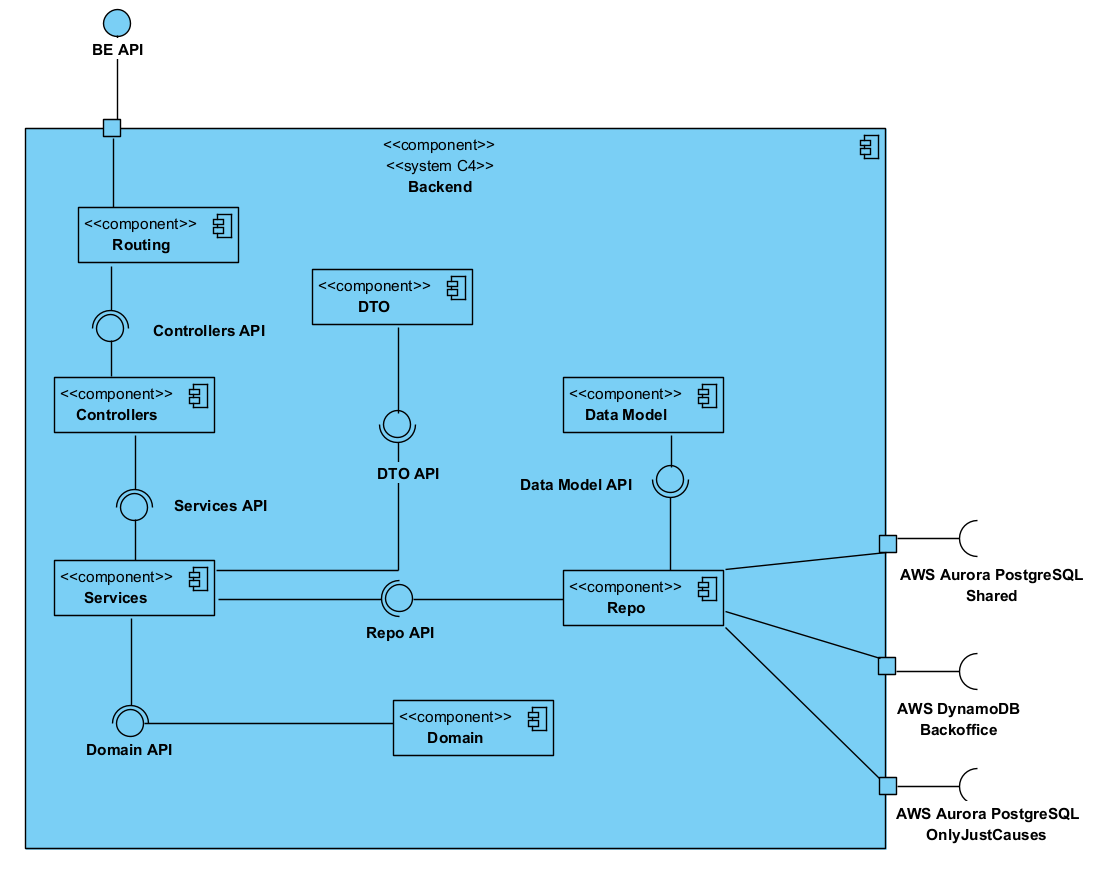
\includegraphics[width=0.95\textwidth, height=0.85\textheight, keepaspectratio]{frontmatter/assets/backoffice/docs/C4-Level3BE.png}
\caption{Diagrama de componentes do \textit{back-end}: C4 Nível 3}
\label{fig:c4_level3_be}
\end{figure}

Depois da Figura~\ref{fig:c4_level3_be}, o ponto a reter é que os módulos não acedem diretamente uns aos outros de forma arbitrária. A autorização entra antes da lógica de negócio, os serviços concentram regras do domínio, os repositórios isolam a persistência e a auditoria acompanha as operações relevantes.

Para além da decomposição por componentes, a implementação do \textit{back-end} seguiu uma separação por camadas. A Figura~\ref{fig:c4_level3_implementation} apresenta essa vista de implementação, centrada na passagem entre rotas, controladores, serviços, repositórios e modelos de domínio. Esta separação reduz o acoplamento entre camadas e permite evoluir módulos sem alterar toda a cadeia de dependências.

\IfFileExists{frontmatter/assets/backoffice/docs/C4-Level3Implementation.png}{
\begin{figure}[H]
\centering
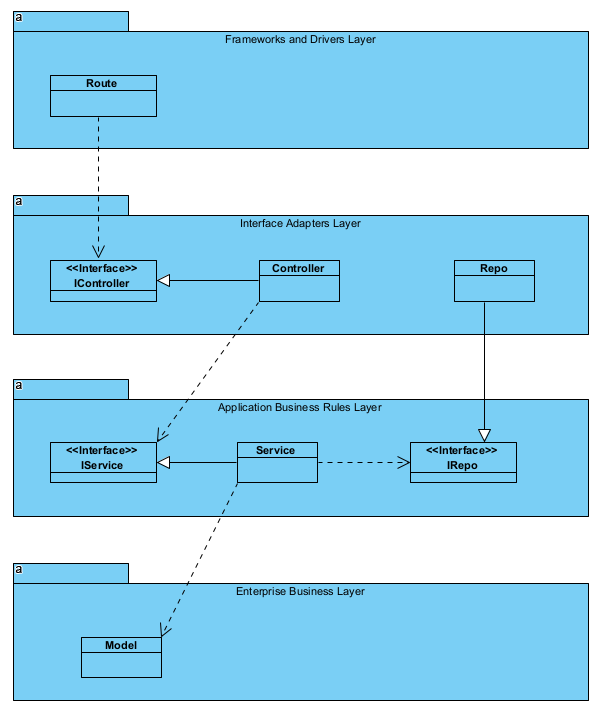
\includegraphics[width=0.9\textwidth, height=0.78\textheight, keepaspectratio]{frontmatter/assets/backoffice/docs/C4-Level3Implementation.png}
\caption{Vista de implementação por camadas}
\label{fig:c4_level3_implementation}
\end{figure}

Depois da Figura~\ref{fig:c4_level3_implementation}, importa perceber a direção das dependências. As rotas pertencem à camada mais externa e encaminham pedidos para controladores. Os controladores adaptam o pedido HTTP para chamadas de serviço. Os serviços concentram as regras de negócio e dependem de interfaces de repositório, não de detalhes concretos de persistência. Os modelos representam os conceitos centrais usados por essas regras. Esta organização ajuda a manter a lógica de negócio protegida de detalhes de infraestrutura.
}{}

\subsubsection{Componentes do \textit{front-end}}

O \textit{front-end} é organizado em páginas e componentes React, com uma camada de serviços responsável pela comunicação com a \gls{API} e uma camada de gestão de estado local. O roteamento é gerido pelo React Router, com proteção de rotas baseada no contexto de acesso devolvido pelo \textit{back-end}: aplicações acessíveis, perfis atribuídos e permissões efetivas. Esta decisão evita que o cliente tenha de reconstruir sozinho regras de autorização a partir do token de autenticação. A Figura~\ref{fig:c4_level3_fe} apresenta esta organização do cliente.

A implementação foi mantida sobre a base React já existente da empresa, em vez de adotar uma ferramenta genérica de administração. Esta decisão preservou o \textit{design system} usado pela OnlyHighIQ e manteve controlo direto sobre fluxos de autorização, auditoria e navegação multiaplicação.

\begin{figure}[H]
\centering
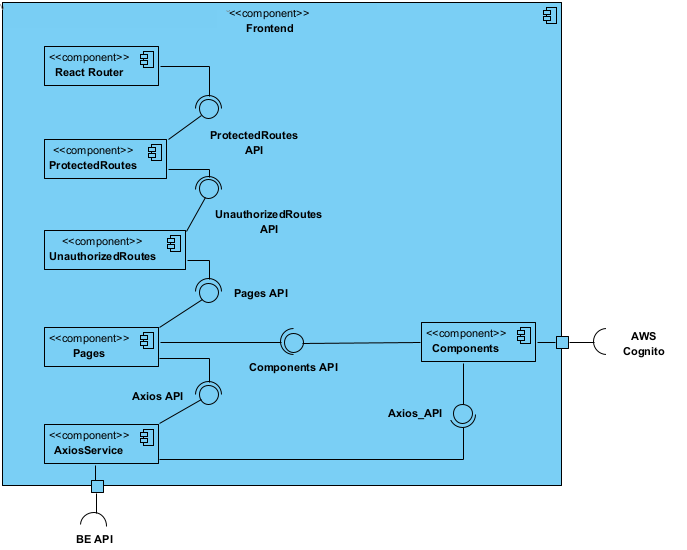
\includegraphics[width=0.95\textwidth, height=0.85\textheight, keepaspectratio]{frontmatter/assets/backoffice/docs/C4-Level3Fe.png}
\caption{Diagrama de componentes do \textit{front-end}: C4 Nível 3}
\label{fig:c4_level3_fe}
\end{figure}

Depois da Figura~\ref{fig:c4_level3_fe}, a leitura pretendida é que a interface não é a fonte final de autorização. O \textit{front-end} melhora a experiência do operador ao esconder páginas e ações indisponíveis, mas trabalha sempre sobre o contexto de acesso calculado no servidor.

\subsubsection{Fluxos de sistema e diagramas de sequência}
\label{sec:diagramas_comportamento}

No Nível 3, os diagramas de componentes explicam a organização interna do \textit{front-end} e do \textit{back-end}. Para completar essa leitura, os \glspl{SSD} seguintes resumem os principais fluxos ao nível da interação entre o operador e o sistema. Os \glspl{SSD} não mostram os componentes internos, mas indicam que pedidos entram no backoffice, que respostas são devolvidas e que decisões do sistema condicionam cada operação. As Figuras~\ref{fig:ssd_login} a~\ref{fig:ssd_kyb_verification} apresentam estes fluxos resumidos; os \glspl{SD} detalhados correspondentes encontram-se no Apêndice~\ref{app:sd_detalhados}, onde cada fluxo é expandido com controladores, serviços, repositórios, persistência e registos de auditoria.

\begin{figure}[H]
\centering

\includegraphics[width=0.9\textwidth, height=0.38\textheight, keepaspectratio]{frontmatter/assets/backoffice/ch3/uml/login-authentication/ssd}
\caption{SSD: autenticação e resolução inicial do operador}
\label{fig:ssd_login}
\end{figure}

Depois da Figura~\ref{fig:ssd_login}, a leitura pretendida é que a autenticação não termina na validação da identidade. O operador inicia a sessão, mas o sistema ainda tem de resolver o utilizador interno, confirmar o estado da conta e calcular o acesso disponível antes de permitir a navegação. O fluxo detalhado encontra-se na Secção~\ref{app:sd_login_full}.

\begin{figure}[H]
\centering

\includegraphics[width=0.9\textwidth, height=0.38\textheight, keepaspectratio]{frontmatter/assets/backoffice/ch3/uml/create-admin-user/ssd}
\caption{SSD: criação de operador administrativo}
\label{fig:ssd_create_admin}
\end{figure}

Depois da Figura~\ref{fig:ssd_create_admin}, a leitura principal é que a criação de operadores administrativos é tratada como uma operação sensível. O sistema valida a autoridade do operador autenticado, cria a conta administrativa, associa o perfil pretendido e regista a ação para auditoria. O detalhe da colaboração interna é apresentado na Secção~\ref{app:sd_create_admin_full}.

\begin{figure}[H]
\centering

\includegraphics[width=0.9\textwidth, height=0.38\textheight, keepaspectratio]{frontmatter/assets/backoffice/ch3/uml/CH4-ROLE-ASSIGNMENT/ssd}
\caption{SSD: atribuição de perfil por aplicação}
\label{fig:ssd_role_assignment}
\end{figure}

Depois da Figura~\ref{fig:ssd_role_assignment}, importa observar que a atribuição de perfis não é uma simples edição de um campo do utilizador. O sistema valida a hierarquia administrativa, a aplicação associada ao perfil, a regra de apenas um perfil por aplicação e a exclusividade dos perfis globais de backoffice. O SD detalhado da Secção~\ref{app:sd_role_assignment_full} mostra onde estas validações são aplicadas.

\begin{figure}[H]
\centering

\includegraphics[width=0.9\textwidth, height=0.38\textheight, keepaspectratio]{frontmatter/assets/backoffice/ch3/uml/roles-permissions/ssd}
\caption{SSD: gestão de perfis e permissões}
\label{fig:ssd_roles_permissions}
\end{figure}

Depois da Figura~\ref{fig:ssd_roles_permissions}, a leitura esperada é que os perfis e permissões são sempre administrados dentro do contexto de uma aplicação. Esta separação impede que permissões de uma aplicação sejam associadas a perfis de outra e suporta a evolução do backoffice para novas aplicações sem alterar o princípio de autorização. A Secção~\ref{app:sd_roles_permissions_full} detalha o carregamento, a edição e a persistência destas alterações.

\begin{figure}[H]
\centering

\includegraphics[width=0.9\textwidth, height=0.38\textheight, keepaspectratio]{frontmatter/assets/backoffice/ch3/uml/CH4-PAGE-GATES/ssd}
\caption{SSD: configuração de page gates}
\label{fig:ssd_page_gates}
\end{figure}

Depois da Figura~\ref{fig:ssd_page_gates}, a leitura principal é que o acesso a páginas é configurável a partir do próprio backoffice. O operador escolhe a aplicação, seleciona a página e define que permissões dão acesso a essa área, enquanto o sistema valida a consistência das permissões e guarda a configuração. O fluxo detalhado é apresentado na Secção~\ref{app:sd_page_gates_full}.

\begin{figure}[H]
\centering

\includegraphics[width=0.9\textwidth, height=0.38\textheight, keepaspectratio]{frontmatter/assets/backoffice/ch3/uml/CH4-USER-ACTIVITY/ssd}
\caption{SSD: consulta de atividade de operador}
\label{fig:ssd_user_activity}
\end{figure}

Depois da Figura~\ref{fig:ssd_user_activity}, observa-se que a consulta de atividade agrega evidências de duas origens: ações administrativas registadas em audit logs e tentativas ou eventos de acesso registados em audit trail. Esta visão ajuda a reconstruir o comportamento de um operador sem expor diretamente a complexidade das tabelas internas. A Secção~\ref{app:sd_user_activity_full} descreve a agregação e a filtragem em detalhe.

\begin{figure}[H]
\centering

\includegraphics[width=0.9\textwidth, height=0.38\textheight, keepaspectratio]{frontmatter/assets/backoffice/ch3/uml/CH4-CAMPAIGN-REVISION/ssd}
\caption{SSD: revisão de campanha}
\label{fig:ssd_campaign_revision}
\end{figure}

Depois da Figura~\ref{fig:ssd_campaign_revision}, a leitura pretendida é que a revisão de campanhas combina decisão operacional e comunicação com o utilizador. O sistema valida a permissão do operador, aplica a decisão ao estado da campanha, regista a ação e, quando aplicável, envia a notificação ou o e-mail associado. A Secção~\ref{app:sd_campaign_revision_full} expande este fluxo.

\begin{figure}[H]
\centering

\includegraphics[width=0.9\textwidth, height=0.38\textheight, keepaspectratio]{frontmatter/assets/backoffice/ch3/uml/manage-categories/ssd}
\caption{SSD: gestão de categorias}
\label{fig:ssd_categories}
\end{figure}

Depois da Figura~\ref{fig:ssd_categories}, a leitura principal é que os módulos operacionais da JustCauses seguem o mesmo padrão arquitetural usado nas funcionalidades transversais do backoffice. O operador pede a listagem ou alteração de categorias, o sistema valida a autorização, executa a operação no domínio da aplicação e regista a ação administrativa. O SD detalhado encontra-se na Secção~\ref{app:sd_categories_full}.

\IfFileExists{frontmatter/assets/backoffice/ch3/uml/kyc-verification/ssd.png}{
\begin{figure}[H]
\centering

\includegraphics[width=0.9\textwidth, height=0.38\textheight, keepaspectratio]{frontmatter/assets/backoffice/ch3/uml/kyc-verification/ssd}
\caption{SSD: verificação KYC de utilizadores individuais}
\label{fig:ssd_kyc_verification}
\end{figure}

Depois da Figura~\ref{fig:ssd_kyc_verification}, a leitura pretendida é que a fila \gls{KYC} não é apenas uma listagem de documentos. O operador consulta submissões, o sistema compara os dados de perfil com os dados recebidos do fornecedor de verificação e, perante inconsistências ou submissões pendentes há demasiado tempo, permite ações controladas, notificadas e auditadas. O SD detalhado encontra-se na Secção~\ref{app:sd_kyc_verification_full}.
}{}

\IfFileExists{frontmatter/assets/backoffice/ch3/uml/kyb-verification/ssd.png}{
\begin{figure}[H]
\centering

\includegraphics[width=0.9\textwidth, height=0.38\textheight, keepaspectratio]{frontmatter/assets/backoffice/ch3/uml/kyb-verification/ssd}
\caption{SSD: verificação KYB de organizações}
\label{fig:ssd_kyb_verification}
\end{figure}

Depois da Figura~\ref{fig:ssd_kyb_verification}, observa-se que a organização é tratada como entidade do domínio da JustCauses e não como uma conta administrativa. O operador abre a submissão \gls{KYB}, consulta os documentos associados, toma uma decisão de aprovação ou rejeição, e o sistema atualiza o estado de verificação, cria notificação, envia e-mail quando aplicável e regista a auditoria. O SD detalhado encontra-se na Secção~\ref{app:sd_kyb_verification_full}.
}{}

\subsubsection{Modelo de dados administrativo}
\label{sec:modelo_dados}

O modelo de dados administrativo descreve apenas a persistência própria do backoffice, mantida em DynamoDB. Os dados transacionais da JustCauses continuam na base relacional da aplicação e são tratados, nesta arquitetura, como uma dependência externa ao modelo administrativo. A Figura~\ref{fig:backoffice_data_model} apresenta as tabelas administrativas que suportam esta camada.

\IfFileExists{frontmatter/assets/backoffice/ch3/uml/architecture/backoffice-data-model.png}{
\begin{figure}[H]
\centering
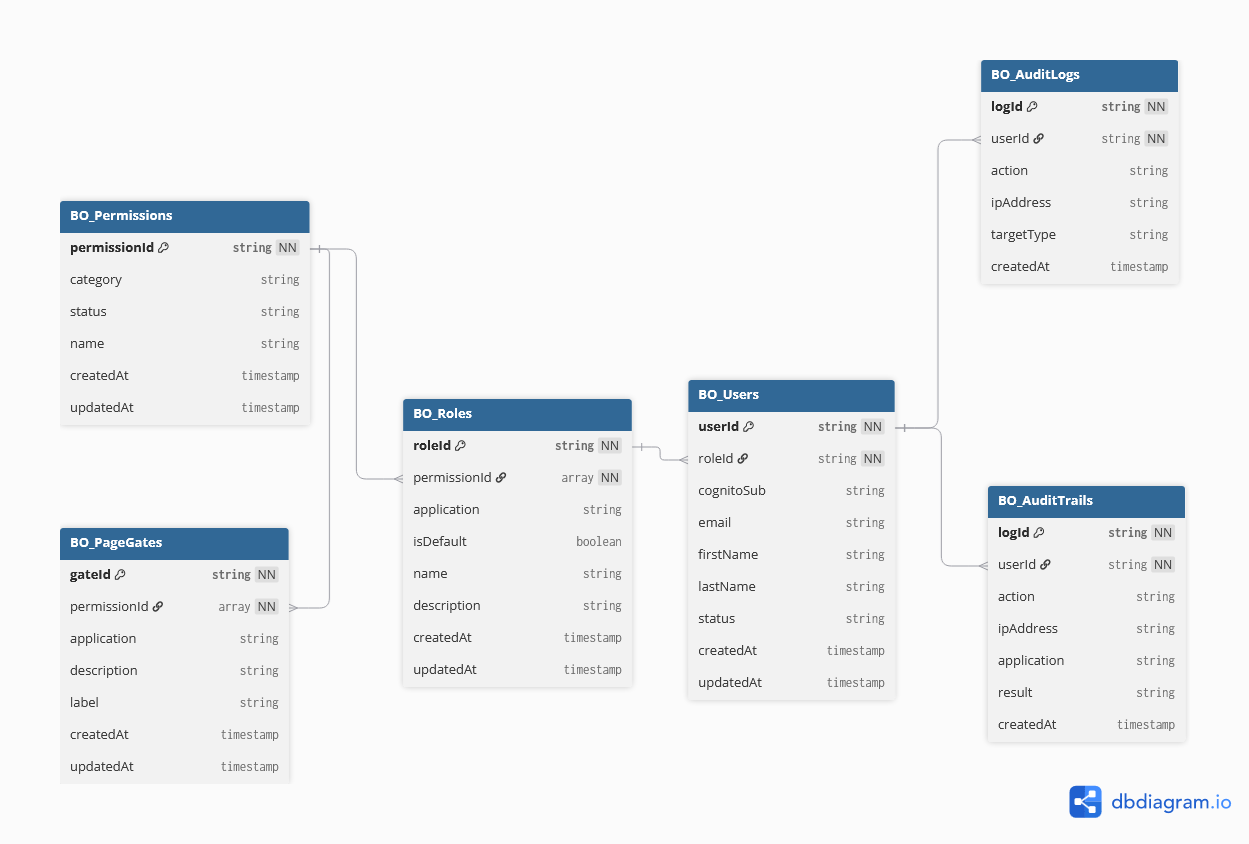
\includegraphics[width=0.95\textwidth, height=0.82\textheight, keepaspectratio]{frontmatter/assets/backoffice/ch3/uml/architecture/backoffice-data-model.png}
\caption{Modelo de dados administrativo do backoffice}
\label{fig:backoffice_data_model}
\end{figure}

Depois da Figura~\ref{fig:backoffice_data_model}, a leitura principal é a centralidade do operador interno no modelo administrativo. A tabela \texttt{BO\_Users} liga a identidade autenticada no Cognito ao perfil ou perfis de acesso configurados no backoffice. As tabelas \texttt{BO\_Roles}, \texttt{BO\_Permissions} e \texttt{BO\_PageGates} suportam a autorização: os perfis agregam permissões, e os \textit{page gates} definem que permissões permitem abrir cada área da aplicação. A auditoria fica associada ao utilizador que executou ou tentou executar a ação através de \texttt{BO\_Logs}. Esta tabela guarda tanto ações administrativas como eventos de acesso, sendo a distinção feita pelo tipo de ação e pelos filtros usados na interface. Esta relação evita registos anónimos dentro do contexto administrativo. A Tabela~\ref{tab:modelo_dados_admin} resume a responsabilidade de cada tabela.
}{}

\begin{table}[H]
\caption{Tabelas administrativas do backoffice em DynamoDB}
\label{tab:modelo_dados_admin}
\begin{center}
\small
\begin{tabular}{|l|p{9cm}|}
\hline
\textbf{Tabela} & \textbf{Responsabilidade} \\ \hline
\texttt{BO\_Users} & Guarda os operadores internos, estado da conta, identificador Cognito, e-mail e referência aos perfis atribuídos. A relação com \texttt{BO\_Roles} deve ser lida em conjunto com a regra funcional de um perfil por aplicação. \\ \hline
\texttt{BO\_Roles} & Guarda os perfis de acesso, cada um associado a uma aplicação e a um conjunto de permissões dessa mesma aplicação. \\ \hline
\texttt{BO\_Permissions} & Guarda as permissões disponíveis para autorização granular, agrupadas por categoria e usadas por perfis e \textit{page gates}. \\ \hline
\texttt{BO\_PageGates} & Guarda a configuração de acesso a páginas por aplicação, incluindo a identificação da página e as permissões aceites para a abrir. \\ \hline
\texttt{BO\_Logs} & Guarda ações administrativas, tentativas de acesso e eventos de autenticação ou navegação relevantes, sempre associados a um utilizador interno, a uma marca temporal e ao contexto necessário para consulta por filtros. \\ \hline
\end{tabular}
\end{center}
\end{table}

Depois da Tabela~\ref{tab:modelo_dados_admin}, a leitura principal é que a escalabilidade do backoffice está concentrada num modelo administrativo próprio. Ao guardar operadores, perfis, permissões, \textit{page gates} e auditoria fora dos dados transacionais da JustCauses, o sistema consegue acrescentar novas aplicações sem misturar configuração transversal com entidades específicas de cada produto. Esta tabela deve ser lida em conjunto com a Figura~\ref{fig:domain_model} e com a Figura~\ref{fig:backoffice_data_model}: o primeiro diagrama mostra o domínio global administrado pelo painel, enquanto o segundo identifica as estruturas persistidas que pertencem ao núcleo administrativo do backoffice.

\subsubsection{Modelo de permissões}
\label{sec:modelo_permissoes}

O modelo de permissões não foi tratado apenas como uma lista de perfis. Na implementação real, a autorização resulta da combinação entre o contexto do operador, a aplicação em causa e a ação concreta pedida ao sistema. A autenticação é comum, mas a autorização é resolvida depois, com base nos dados internos do backoffice.

Em termos práticos, há dois grandes contextos de utilização: o backoffice de gestão e o painel operacional da JustCauses. Ambos partilham a mesma autenticação Cognito, mas o acesso efetivo é refinado por três decisões sucessivas: acesso à aplicação, acesso à página e autorização da ação pedida à \gls{API}. Esta decomposição permite alinhar a interface, o \textit{router}, o \textit{middleware} da \gls{API} e o sistema de auditoria sob a mesma regra de negócio.

Assim, o desenho do modelo de permissões responde a quatro perguntas principais: o operador autenticado pode entrar na aplicação pedida; pode abrir a página para a qual foi encaminhado; pode executar a ação disponível na interface; e o servidor deve aceitar ou rejeitar o pedido \gls{HTTP} correspondente.

Quando o operador inicia sessão, o token do Cognito identifica a sessão, mas não chega para decidir o acesso às áreas internas. O \textit{back-end} localiza o registo do utilizador interno, verifica se a conta está ativa e resolve os perfis associados ao campo \texttt{roleIds}. O campo antigo \texttt{roleId} mantém-se apenas como compatibilidade com dados legados e representa, quando existe, o primeiro perfil do utilizador.

O modelo atual permite que um operador tenha zero ou mais perfis aplicacionais, mas impõe duas regras: só pode existir um perfil por aplicação e um perfil de backoffice é exclusivo, não podendo ser combinado com perfis aplicacionais. As permissões também têm uma aplicação associada; por isso, uma permissão da JustCauses não pode ser atribuída a um perfil de backoffice, e o servidor rejeita essa configuração mesmo que a interface tente enviá-la.

Depois de resolver os perfis, o servidor calcula o acesso efetivo: lista de perfis, permissões globais, permissões agrupadas por aplicação e aplicações acessíveis. Esta resolução centralizada evita que cada página tenha de interpretar o modelo de autorização de forma diferente.

A Tabela~\ref{tab:camadas_autorizacao} resume as camadas em que a autorização é aplicada.

\begin{table}[H]
\caption{Camadas de aplicação do modelo de autorização}
\label{tab:camadas_autorizacao}
\begin{center}
\small
\begin{tabular}{|p{3cm}|p{3.4cm}|p{7cm}|}
\hline
\textbf{Camada} & \textbf{Fonte de decisão} & \textbf{Regra aplicada} \\ \hline
Resolução do contexto & Cognito + \texttt{BO\_Users} + \texttt{BO\_Roles} + \texttt{BO\_Permissions} & O sistema valida o token, confirma o estado da conta, resolve os perfis atribuídos e calcula permissões efetivas por aplicação. \\ \hline
Guardas de rota & React Router & \texttt{ProtectedRoute} exige sessão; \texttt{BackofficeRoute} e \texttt{PanelRoute} usam a lista de aplicações acessíveis para decidir a entrada. \\ \hline
Acesso a páginas & \texttt{BO\_PageGates} & Cada página declara as permissões mínimas necessárias; quando há várias permissões, aplica-se lógica OR. \\ \hline
Ações na interface & \texttt{usePermission} & Botões e ações sensíveis só são apresentados quando a permissão necessária existe no contexto do utilizador. \\ \hline
\gls{API} & \texttt{requirePermission} & O servidor revalida permissões antes de executar a operação, devolve \texttt{401}/\texttt{403} quando necessário e regista acessos negados. \\ \hline
\end{tabular}
\end{center}
\end{table}

Depois da Tabela~\ref{tab:camadas_autorizacao}, o que se deve retirar é que a autorização é deliberadamente redundante. A interface filtra aplicações, páginas e ações para guiar o operador, mas a \gls{API} revalida os pedidos antes de alterar dados. Esta opção foi escolhida para evitar que a segurança dependesse apenas do cliente.

Existem também regras de exceção explícitas. O Super Admin recebe todas as permissões efetivas e mantém a capacidade de administração global. Os perfis de backoffice, incluindo o Backoffice Admin, têm acesso global às aplicações fora do próprio backoffice, mas só recebem permissões administrativas de backoffice quando estas estão guardadas no respetivo perfil, mantendo ainda as restrições já definidas para ações sobre utilizadores de nível equivalente ou superior. Em sentido inverso, um perfil associado apenas a \texttt{just\_causes} não pode entrar no backoffice administrativo. Um operador sem perfis atribuídos fica autenticado, mas sem acesso funcional a aplicações internas.

Esta opção evita uma matriz estática demasiado rígida. Em vez de fixar todas as relações entre perfis e páginas no código, as permissões disponíveis, os perfis e os \textit{page gates} ficam persistidos no DynamoDB, nas tabelas \texttt{BO\_Permissions}, \texttt{BO\_Roles} e \texttt{BO\_PageGates}. Como cada perfil e cada permissão têm uma aplicação associada, a integração de uma nova aplicação segue o mesmo padrão conceptual: definir permissões da aplicação, criar perfis dessa aplicação e configurar os respetivos \textit{page gates}.

%----------------------------------------------------------------------------------------

\section{Sumário}
\label{sec:sumario_cap3}

Este capítulo descreveu os requisitos, a análise do domínio, a arquitetura e o desenho do backoffice multiaplicação, tendo a JustCauses como primeira aplicação operacional integrada. A análise concentrou-se nos mecanismos que sustentam o comportamento do sistema: separação entre aplicações, resolução centralizada de permissões, \textit{page gates}, auditoria e revalidação no \textit{back-end}. Os requisitos funcionais foram organizados em treze capacidades centrais, com destaque para autenticação, autorização, operação da plataforma, verificação \gls{KYC}/\gls{KYB} e rastreabilidade. A arquitetura adotada, descrita com recurso a C4+1, separa o \textit{front-end} React do \textit{back-end} Node.js, com persistência em \gls{PostgreSQL} e DynamoDB e infraestrutura na AWS. O modelo de permissões é tratado como um mecanismo transversal que decide, em cada pedido, as aplicações, páginas e ações acessíveis ao operador. O capítulo seguinte descreve como esse desenho foi concretizado no código e na interface.
